\documentclass[12pt]{article}

\usepackage{amsmath, amssymb, amsthm, mathrsfs, fancyhdr}
\usepackage{syntonly, lastpage, hyperref, enumitem, graphicx}
%\usepackage[style=authoryear]{biblatex}
\usepackage{booktabs}
\usepackage{float}

\usepackage{amsmath, amsthm, mathtools,commath}
\usepackage{graphics, color}
\usepackage{latexsym}
\usepackage{amssymb, amsfonts, bm}
\usepackage{mathrsfs}

\usepackage{graphicx}
\usepackage{epsfig}
\usepackage{makeidx}
\usepackage{fullpage}
\usepackage{booktabs, arydshln}
\usepackage{comment} 
%\makeindex

\hbadness=10000 \tolerance=10000 \hyphenation{en-vi-ron-ment
in-ven-tory e-num-er-ate char-ac-ter-is-tic}

\usepackage[round]{natbib}
%\bibliographystyle{apalike2}
% \bibliographystyle{jmr}


\newcommand{\biblist}{\begin{list}{}
{\listparindent 0.0cm \leftmargin 0.50cm \itemindent -0.50 cm
\labelwidth 0 cm \labelsep 0.50 cm
\usecounter{list}}\clubpenalty4000\widowpenalty4000}
\newcommand{\ebiblist}{\end{list}}

\newcounter{list}

%\usepackage{setspace}

%\usepackage{hangpar}
\newcommand{\lbl}[1]{\label{#1}{\ensuremath{^{\fbox{\tiny\upshape#1}}}}}
% remove % from next line for final copy
\renewcommand{\lbl}[1]{\label{#1}}

\newtheorem{theorem}{Theorem}
\newtheorem{corollary}{Corollary}
\newtheorem{definition}{Definition}
\newtheorem{example}{Example}
\newtheorem{remark}{Remark}
\newtheorem{result}{Result}

\newtheorem{lemma}{Lemma}

\DeclareMathOperator*{\argmin}{arg\,min}
\DeclareMathOperator*{\argmax}{arg\,max}
\newcommand{\MAP}{{\text{MAP}}}
\newcommand{\Cov}{{\text{Cov}}}
\newcommand{\Var}{{\text{Var}}}
\newcommand{\logistic}{{\text{logistic}}}

\newcommand{\bx}{\mathbf{x}}
\newcommand{\R}{\mathbb{R}}
\renewcommand{\bf}[1]{\mathbf{#1}}


\begin{document}

\title{Similarities between Nonnested Regression Estimation and Ridge Regression}
\author{Caleb Leedy}
\maketitle 

\baselineskip .3in

\section{Nonnested Regression}

In the case of non-nested two phase sampling, we have $A_1 = (X_i)_{i = 1}^{n_1}$
and $A_2 = (X_1, Y_i)_{i = 1}^{n_2}$ with $A_1$ and $A_2$ being selected
independently from the same sampling frame. The regression estimator is then

\begin{align*}
\hat{\bar{Y}}_{reg} 
  &= \hat{\bar{Y}}_{HT} + (\hat{\bar{X}}_c - \hat{\bar{X}}_2)' \hat \beta_2 
  & \text{for } \hat \beta_2 = \left(\sum_{i \in A_2} x_i x_i'\right)^{-1} 
    \sum_{i \in A2} x_i y_i \text{ with } x_{1i} = 1 \\
  &= \hat{\bar{Y}}_{HT} + (\hat{\bar{X}}_1 - \hat{\bar{X}}_2)'W'\hat \beta_2 
  & \text{ if } \hat{\bar{X}}_c = W \hat{\bar{X}}_1 + (I - W) \hat{\bar{X}}_2\\
  &= \sum_{i \in A_1} x_i' W' \hat \beta_2 + \sum_{i \in A_2} (y_i - x_i' W'
  \hat \beta_2).
\end{align*}

While the matrix $W$ controls the interaction between $A_1$ and $A_2$ it also
plays the role of shrinkage on $\hat \beta_2$.


\textcolor{red}{If the population total of $X$ is known, then the regression
  estimator 
  $$ \hat{\bar{Y}}_{reg} = \hat{\bar{Y}}_{HT} + ({\bar{X}} - \hat{\bar{X}}_2)' \hat \beta_2$$
  can be used. In this case, $\hat{\beta}_2$ does not have the shrinkage
  interpretation. Now, if $\bar{X}$ is unknown, we need to use an estimator. If
  we use the best estimator $\hat{\bar{X}}_c$, then the residual is orthogonal.
  Otherwise, if we use an inefficient estimator $\hat{\bar{X}}_1$, we pay its
  price. It is more related to attenuation effect in the measurement error model
  problem. 
}

\section{Ridge Regression}

Given a sample $A$, ridge regression solves the optimization problem,

$$\hat \beta = \argmin_{\beta \in \R^p} \sum_{i \in A} (y_i - x_i'\beta)^2 + \beta^T
(\lambda I_p) \beta.$$

Differentiating with respect to $\beta$ and setting this equal to zero yields a
solution,

$$\hat \beta = \left(\sum_{i \in A} x_i x_i' + \lambda I_p\right)^{-1} \sum_{i
\in A} x_i' y_i = (X'X + \lambda I_p)^{-1} X'Y.$$

Let $\hat \beta_{OLS} = \hat \beta_2 = (X'X)^{-1} X'Y$, then using the
Sherman-Morrison-Woodbury inverse formula,

$$\hat \beta = (I_p - (X'X)^{-1}(\lambda^{-1}I_p + (X'X)^{-1}))^{-1} \hat \beta_{OLS}.$$

\section{Discussion}

The previous two sections suggest that if we let

$$
\begin{aligned}
  W &= (I_p - (X'X)^{-1}(\lambda^{-1}I_p + (X'X)^{-1}))^{-1} \\
  \iff \lambda W &= (X'X)(I_p - W) \\ 
  \iff \lambda &= (X'X)(W^{-1} - I_p)
\end{aligned}
$$

then we would have equivalent results. In this way, non-nested two phase
sampling is like ridge regression.

\begin{itemize}
  \item We could connect this to LASSO?
  \item This could be a connection to Bayesian statistics and choosing priors on
    our estimates?
  \item Maybe this can help us choose priors for ridge regression better?
\end{itemize}


\section{Alternative idea for non-parametric regression estimation}

One possible idea is to develop a debiased estimation under two-phase sampling.
If the covariates are high dimensional or the regression employs nonparametric
regression (such as spline or random forest, etc), then the resulting two-phase
regression estimator can be biased. To correct for the bias, we can use the
following approach.

\begin{enumerate}
\item Split the sample $A_2$ into two parts: $A_2= A_2^{(a)} \cup A_2^{(b)}$.
  We can use SRS to split the sample, but other sampling designs can be used. 

\item Use the observations in $A_2^{(a)}$ only to obtain a predictor of $y_i$,
  $\hat{f}^{(a)} (\bx_i)$. Also, use the observations in $A_2^{(b)}$ only to
  obtain a predictor of $y_i$, $\hat{f}^{(b)} (\bx_i)$. 

\item Let 
$$ \hat{f}(\bx_i) = \left( \hat{f}^{(a)} (\bx_i) + \hat{f}^{(b)} (\bx_i) \right)/ 2$$
be the predictor combining two samples. 

\item The final debiased two-phase regression estimator is given by 
\begin{equation}
\hat{Y}_{\rm d, reg} = \sum_{i \in A_1} w_{1i}  \hat{f}(\bx_i) +  
\sum_{i \in A_2^{(a)} } w_{1i} \pi_{2i \mid 1}^{-1} \left\{y_i - \hat{f}^{(b)} (\bx_i) \right\} +
\sum_{i \in A_2^{(b)} } w_{1i} \pi_{2i \mid 1}^{-1} \left\{y_i - \hat{f}^{(a)} (\bx_i) \right\}
\label{debiased}
\end{equation}
\end{enumerate}

 If I am not mistaken, there are several advantages of the debiased two-phase
 regression estimator in (\ref{debiased}). 

\begin{enumerate}
\item Unlike the classical two-phase regression estimator using nonparametric
  regression, we can establish asymptotic unbiasedness and
  $\sqrt{n}$-consistency. 
\item Even if we use the sample split, there is no efficiency loss. That is, the
  asymptotic variance is equal to 

$$ V \left( \hat{Y}_{\rm d, reg} \right) = V \left( \hat{Y}_1 \right) + E\left[
V \left\{ \sum_{i \in A_2} w_{1i} \pi_{2i \mid 1}^{-1} \left( y_i - f(\bx_i)
\right) \mid A_1 \right\} \right] 
$$

where $f(\bx_i)$ is the probability limit of $\hat{f}(\bx_i)$. 

\item Variance estimation is also straightforward. We can compute 

$$ \hat{\eta}_i = \hat{f}(\bx_i) +\delta_i  \pi_{2i \mid 1}^{-1} I_i^{(a)}
\left\{ y_i - \hat{f}^{(b)}(\bx_i) \right\} +\delta_i \pi_{2i \mid 1}^{-1}
I_i^{(b)} \left\{ y_i - \hat{f}^{(a)} (\bx_i) \right\}$$

and apply to the variance estimation formula for the first-phase sample, 
where $I_i^{(a)}$ is the indicator function for $A_2^{(a)}$ such that $I_i^{(a)}
= 1$ if $i \in A_2^{(a)}$ and $I_i^{(a)}=0$ otherwise. Also, $I_i^{(b)}= 1-
I_i^{(a)}$. 
\end{enumerate}

I also have an idea on how to implement the above debiased regression estimator
using calibration. I will give more details once we are confident in the
proposed idea. 

\subsection{Simulation Study}

We generate a finite population of size $N = 10,000$ from a superpopulation
model of:

$$\begin{aligned}
X_i &\stackrel{ind}{\sim} N(0, 1) \\
\varepsilon_i &\stackrel{ind}{\sim} N(0, 1) \\
Y_i = m(x) + 0.3 \varepsilon_i
\end{aligned}
$$

for $m(x) = 0.2 x + \sin(x)$.
The Phase 1 sample is a simple random sample (SRS) of size $n_1 = 2000$
from the finite population and the Phase 2 sample is a Poisson sample with the
probability of selection into the Phase 2 sample from the Phase 1 sample being
$\max(\min(0.7, \Phi(X_i - 0.5)), 0.02)$ where $\Phi$ is the CDF function of a
normal distribution. These sampling probabilities yield $E[n_2] \approx 700$.

The goal of this simulation is to estimate $\theta = E[Y]$, which is challenging
because $Y$ is a nonlinear function of $X$ as seen in Figure~\ref{fig:popplot}
and Figure~\ref{fig:p2plot}.

\begin{figure}[ht!]
  \centering
  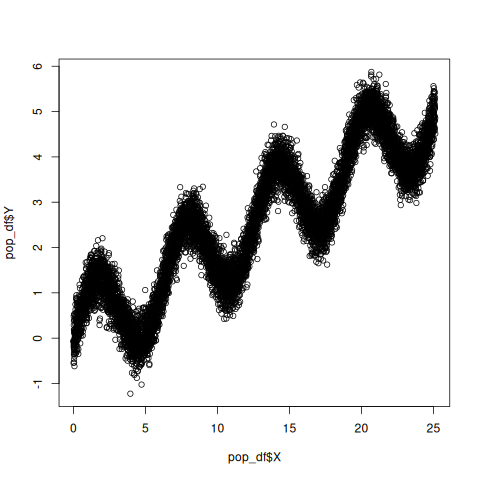
\includegraphics[width=0.5\textwidth]{tables/popplot.png}
  \caption{Population plot of relationship between $X$ and $Y$.}
  \label{fig:popplot}
\end{figure}

\begin{figure}[ht!]
  \centering
  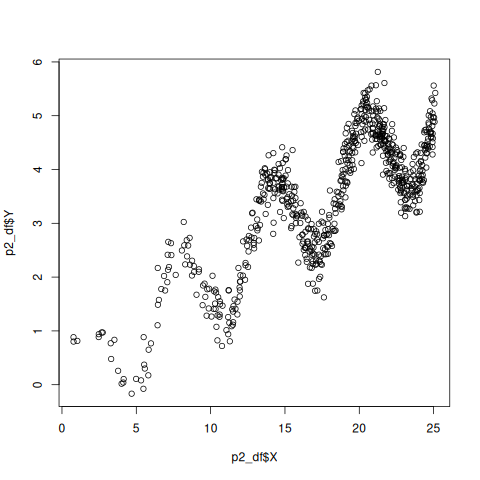
\includegraphics[width=0.5\textwidth]{tables/p2plot.png}
  \caption{Phase 2 plot of relationship between $X$ and $Y$.}
  \label{fig:p2plot}
\end{figure}

We estimate $\theta$ using the estimator:

$$\hat Y = \sum_{i \in A_1} \frac{\hat \eta_i}{\pi_{1i}}$$

where $\hat \eta_i$ differs between three methods:

\begin{itemize}
  \item[1.] Oracle: $\hat \eta_i = m(x_i) + \frac{\delta_{2i|1}}{\pi_{2i|1}}(y_i
    - m(x_i))$ and $m(x)$ is the true mean function of $Y$.
  \item[2.] Naive: $\hat \eta_i = \hat m(x_i) + \frac{\delta_{2i|1}}{\pi_{2i|1}}(y_i
    - \hat m(x_i))$ where $\hat m(x)$ is estimated using the data from the Phase 2
    sample using nonparametric regression. 
  \item[3.] Proposed: $\hat \eta_i = \hat m(x_i) + 
    \frac{\delta_{2i|1}\delta_i^{(a)}}{\pi_{2i|1}}(y_i - \hat m^{(b)}(x_i)) +
    \frac{\delta_{2i|1}\delta_i^{(b)}}{\pi_{2i|1}}(y_i - \hat m^{(a)}(x_i))$
    where $\hat m(x) = \frac 1 2 (\hat m^{(a)}(x) + \hat m^{(b)}(x))$ and $\hat
    m^{(a)}(x)$ is the nonparametric model estimated using $A_2^{(a)}$ and $\hat
    m^{(b)}(x)$ is the nonparametric model estimated using $A_2^{(b)}$. We also
    have $\delta_i^{(a)}$ and $\delta_i^{(b)}$ which denote is $i \in A_2$ was
    part of $A_2^{(a)}$ or $A_2^{(b)}$ respectively.
\end{itemize}

For the Naive and Proposed methods, we use three nonparametric regression
estimators: loess, random forest, and a smoothing spline. These functions come
from the \texttt{stats}, \texttt{randomForest}, and \texttt{npreg} packages in
\texttt{R}. To estimate the variance we use the following:

$$\hat V = \hat S^2_\eta / n_1$$

where $\hat S^2_\eta$ is the estimated variane of $\hat \eta$ in $A_1$.
%\begin{table}[ht!]
%  \begin{tabular}{lrr}
%    \toprule
%    Method & Estimated Variance & Notes \\
%    \midrule
%    Oracle & $\hat V = (\hat V_1 + \hat V_2) / N^2$ & 
%    $\hat V_1 = N^2\left(n_1^{-1} - N^{-1}\right) \hat S_{\eta}$ \\
%           & & $\hat V_2 = \sum_{i \in A_2} 
%           \frac{(1 - \pi_{2i|1})(y_i - m(x_i))^2}{\pi_{1i} \pi_{2i|1}^2}$\\
%    Naive & $\hat V = (\hat V_1 + \hat V_2) / N^2$ & Same as Oracle with $\hat m(x)$
%    instead of $m(x)$.\\
%    Proposed & $\hat V = (\hat V_1 + \hat V_{2a} + \hat V_{2b} + \hat V_{2ab}) / N^2$ 
%             & $\hat V_1$ is the same as $\hat V_1$ from Naive. \\
%             & & $\hat V_{2a} = \frac{1}{4}\sum_{i \in A_2}\sum_{i \in A_2}
%             \frac{\Delta_{2ij|1} + \pi_{2ij|1}}{\pi_{1ij}\pi_{2ij|1}} 
%             \frac{\varepsilon_i^{(b)}}{\pi_{2i|1}}
%             \frac{\varepsilon_j^{(b)}}{\pi_{2j|1}}$\\
%             & & $\hat V_{2b} = \frac{1}{4}\sum_{i \in A_2}\sum_{i \in A_2}
%             \frac{\Delta_{2ij|1} + \pi_{2ij|1}}{\pi_{1ij}\pi_{2ij|1}} 
%             \frac{\varepsilon_i^{(a)}}{\pi_{2i|1}}
%             \frac{\varepsilon_j^{(a)}}{\pi_{2j|1}}$\\
%             & & {\scriptsize$\hat V_{2ab} = 
%             \sum\limits_{i \in A_2} \sum\limits_{i \in A_2} \frac{n_2^{(a)} 
%             \varepsilon_i^{(b)} \varepsilon_j^{(a)}}{n_2
%             \pi_{2ij|1}\pi_{1ij}} \left(\frac{n_2 - n_2^{(a)}}{n_2 - 1}
%             I(i \neq j) - \frac{1 - n_2^{(a)}}{n_2}\right)$}\\
%             & & $\varepsilon_i^{(a)} = (y_i - m^{(a)}(x_i))$,
%             $\varepsilon_i^{(b)} = (y_i - m^{(b)}(x_i))$ \\
%    \bottomrule
%  \end{tabular}
%\end{table}

The results of this simulation for the mean are displayed in
Table~\ref{tbl:npmean} and the variance results are in Table~\ref{tbl:npvar}.

\begin{table}[ht!]
  \centering
  
\begin{tabular}{lrrrr}
\toprule
Est & Bias & RMSE & EmpCI & Ttest\\
\midrule
Oracle & 0.000 & 0.038 & 0.942 & 0.030\\
NaiveLoess & -0.006 & 0.061 & 0.923 & 2.985\\
PropLoess & 0.000 & 0.062 & 0.944 & 0.023\\
NaiveRF & 0.001 & 0.042 & 0.885 & 0.681\\
PropRF & -0.001 & 0.047 & 0.948 & 0.373\\
NaiveSpline & 0.010 & 0.052 & 0.857 & 6.242\\
PropSpline & 0.001 & 0.106 & 0.924 & 0.269\\
\bottomrule
\end{tabular}
  \caption{This shows the results of our simulation. The Est column displays the
  name of the estimator with examples of NaiveLoess indicating the Naive method
  with the loess nonparametric estimator. The Bias column computes $E_{MC}(\hat
  \theta) - \theta_N$ where $E_{MC}$ is the Monte Carlo mean of the 1000
  simulations and $\theta_N$ is the true value from the population. The RMSE
  column computes $\sqrt{B^{-1}\sum_{b = 1}^B (\hat \theta^{(b)} - \theta_N)^2}$
  where $\hat \theta^{(b)}$ is the estimate of $\theta_N$ for the $b$th
  iteration of the Monte Carlo sample. The EmpCI column indicates the fraction
  of iterations for which $|\hat \theta^{(b)} - \theta_N| < 1.96 * \sqrt{\hat V^{(b)}}$
  is true where $\hat V^{(b)}$ is the estimated variance of $\hat \theta^{(b)}$.
  The final column of Ttest gives the test statistic of a test for the bias of the
  estimator being zero.}
  \label{tbl:npmean}
\end{table}

\begin{table}[ht!]
  \centering
  
\begin{tabular}{lrrrr}
\toprule
Est & MCVar & EstVar & VarVar & Ttest\\
\midrule
Oracle & 0.0014 & 0.0013 & 0.0000000 & 16.8\\
NaiveLoess & 0.0037 & 0.0033 & 0.0000006 & 15.4\\
PropLoess & 0.0039 & 0.0042 & 0.0000021 & 6.1\\
NaiveRF & 0.0018 & 0.0012 & 0.0000000 & 143.3\\
PropRF & 0.0022 & 0.0023 & 0.0000005 & 6.0\\
NaiveSpline & 0.0026 & 0.0013 & 0.0000000 & 246.6\\
PropSpline & 0.0113 & 0.0068 & 0.0010567 & 4.4\\
\bottomrule
\end{tabular}
  \caption{This displays the variance results from the simulation. The MCVar
  colum is the Monte Carlo variance of $\hat \theta^{(b)}$ while the EstVar
  column is the average of the estimated variance $\hat V^{(b)}$. The VarVar
  column is the Monte Carlo variance of the variance estimator and the Ttest
  column tests for equality of MCVar and EstVar.}
  \label{tbl:npvar}
\end{table}

Overall, these results seem very promising. From Table~\ref{tbl:npmean}, we can
see the there is evidence for bias in the naive algorithm in both the random
forest and the spline method. Yet, this bias is no longer there under the
proposed method and the empirical confidence intervals are approximately
correct. A further investigation of the variance in Table~\ref{tbl:npvar}
indicates that the estimated variance for the proposed method is too large when
the regression function is either the random forest or smoothing spline, but we
might be approximately correct.

For this simulation, we are still doing well. The only problem is that the naive
method is also working well (especially for the random forest). Maybe I can
choose a more nonlinear function to estimate?

\subsubsection{Simulation Update}

I updated the simulation so that we use the same approach as
\cite{wang2023statistical}. They use a multivariate approach with $X_{1i}$,
$X_{2i}$, $X_{3i}$, and $X_{4i}$ being simulated independently from a $U(1, 3)$
distribution. They have three models for $Y$,

\begin{table}[ht!]
\centering
\begin{tabular}{lr}
\toprule
Model & $Y$ \\
\midrule
A & $Y_i = 3 + 2.5 x_{1i} + 2.75 x_{2i} + 2.5 x_{3i} + 2.25 x_{4i} + \sqrt{3} \varepsilon_i$ \\
B & $Y_i = 3 + (1/35) x_{1i}^2 x_{2i}^3 x_{3i} + 0.1 x_{4i} + \sqrt{3} \varepsilon_i$\\
C & $Y_i = 3 + (1/180) x_{1i}^2 x_{2i}^3 x_{3i} x_{4i}^2 + \sqrt{3} \varepsilon_i$ \\ 
\bottomrule
\end{tabular}
\end{table}

The first phase sample is a SRS with $n_1 = 1000$ and the second phase sample is
a Poisson sample with $\pi_{2i|1} = \logistic(\bf x_i^T \bm \beta + 2.5)$ for $\bm
\beta = (-1.1, 0.5, -0.25, -0.1)^T$. We have modified the spline method to be a
cubic spline with 15 knots for each coordinate and implemented by the \texttt{mgcv}
package. Table~\ref{tbl:np2mean} shows the results
of the simulation under Model C. The results for Model B are similar.

\begin{table}[ht!]
  \centering
  
\begin{tabular}{lrrrr}
\toprule
Est & Bias & RMSE & EmpCI & Ttest\\
\midrule
Oracle & -0.002 & 0.108 & 0.950 & 0.584\\
NaiveLoess & -0.001 & 0.110 & 0.942 & 0.379\\
PropLoess & -0.001 & 0.111 & 0.964 & 0.241\\
NaiveRF & -0.020 & 0.116 & 0.900 & 5.466\\
PropRF & 0.004 & 0.119 & 0.972 & 0.930\\
NaiveSpline & 0.000 & 0.121 & 0.945 & 0.014\\
PropSpline & 0.000 & 0.121 & 0.961 & 0.058\\
\bottomrule
\end{tabular}
  \caption{This shows the results of our simulation. The Est column displays the
  name of the estimator with examples of NaiveLoess indicating the Naive method
  with the loess nonparametric estimator. The Bias column computes $E_{MC}(\hat
  \theta) - \theta_N$ where $E_{MC}$ is the Monte Carlo mean of the 1000
  simulations and $\theta_N$ is the true value from the population. The RMSE
  column computes $\sqrt{B^{-1}\sum_{b = 1}^B (\hat \theta^{(b)} - \theta_N)^2}$
  where $\hat \theta^{(b)}$ is the estimate of $\theta_N$ for the $b$th
  iteration of the Monte Carlo sample. The EmpCI column indicates the fraction
  of iterations for which $|\hat \theta^{(b)} - \theta_N| < 1.96 * \sqrt{\hat V^{(b)}}$
  is true where $\hat V^{(b)}$ is the estimated variance of $\hat \theta^{(b)}$.
  The final column of Ttest gives the test statistic of a test for the bias of the
  estimator being zero.}
  \label{tbl:np2mean}
\end{table}

Unfortunately, with this simulation (and also the simulation with Model B but
not shown here), the naive models are not biased for the loess and spline
methods. It does look like we can debias the result for the random forest
though.

\newpage 

\bibliographystyle{chicago}
\bibliography{references}

\end{document}
